Dato che creare e trainare un buon modello di machine learning non è semplice, nell’elaborato è stato inserito il supporto di una piattaforma per la progettazione e lo studio di modelli, tale applicativo si chiama Tensorboard.

Tensorboard è un set di tool presenti nella libreria di Tensorflow che aiuta l’utilizzatore a capire, ottimizzare e debuggare il suo modello. Ci si accede tramite interfaccia web, basta lanciare in un terminale il comando \texttt{tensorboard --logdir=cartella\_log} per avviare il server web che espone l’interfaccia. Si può quindi utilizzare quest’ultima per visualizzare vari grafici relativi al modello selezionato, visionare parametri, indici, metriche e molto altro.

\begin{figure}[h]
  \centering
  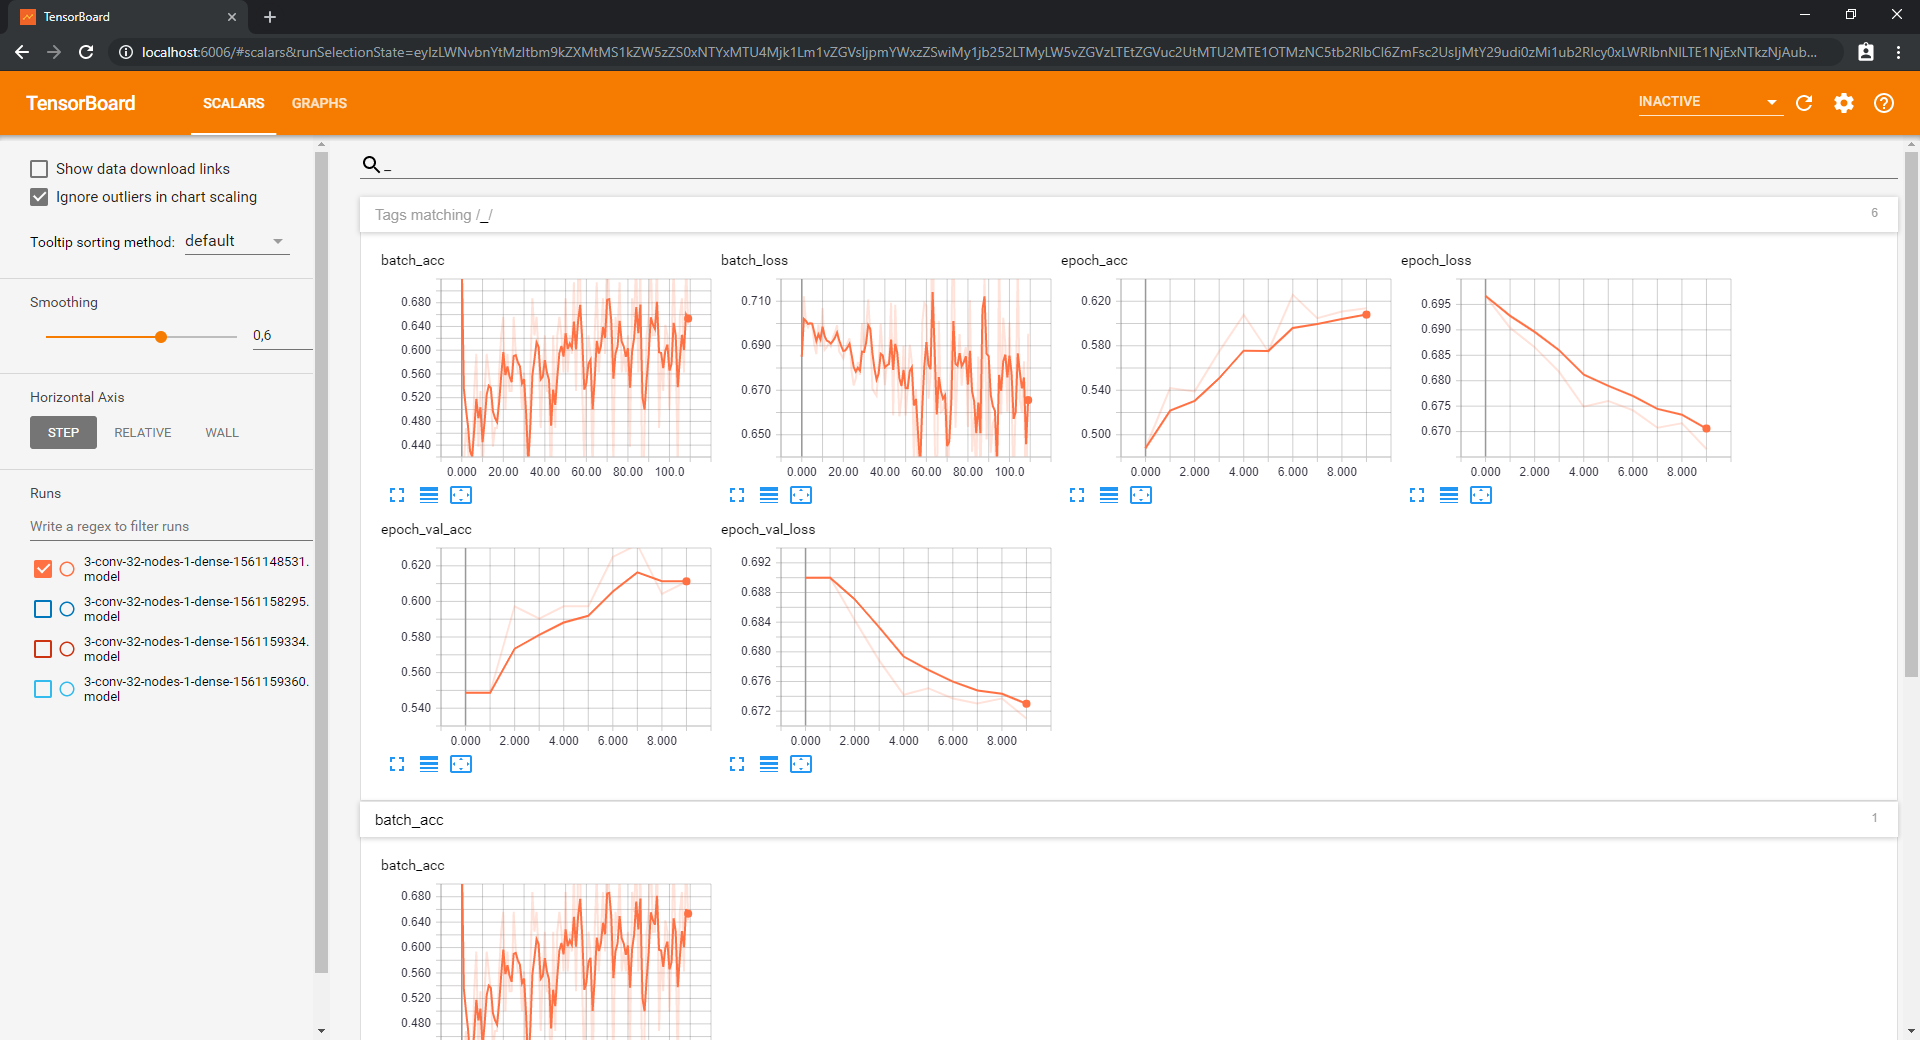
\includegraphics[scale=0.2]{tensorboard.png}
  \caption{Interfaccia iniziale di Tensorboard}
\end{figure}

Quindi questo strumento risulta molto utile per effettuare un'analisi dettagliata su come vari modelli sono composti e soprattutto su come performano. Ad esempio già nella schermata principale si può notare l’andamento dei principali parametri, loss e accuracy, per epoch o per batch. Inoltre navigando nella sezione \texttt{graph} tensorflow fornisce una visualizzazione a grafo del modello, ovvero vengono visualizzati i vari layers della rete specificando le loro connessioni e le variazioni di shape dei dati che passano attraverso la struttura.

\begin{figure}[H]
  \centering
  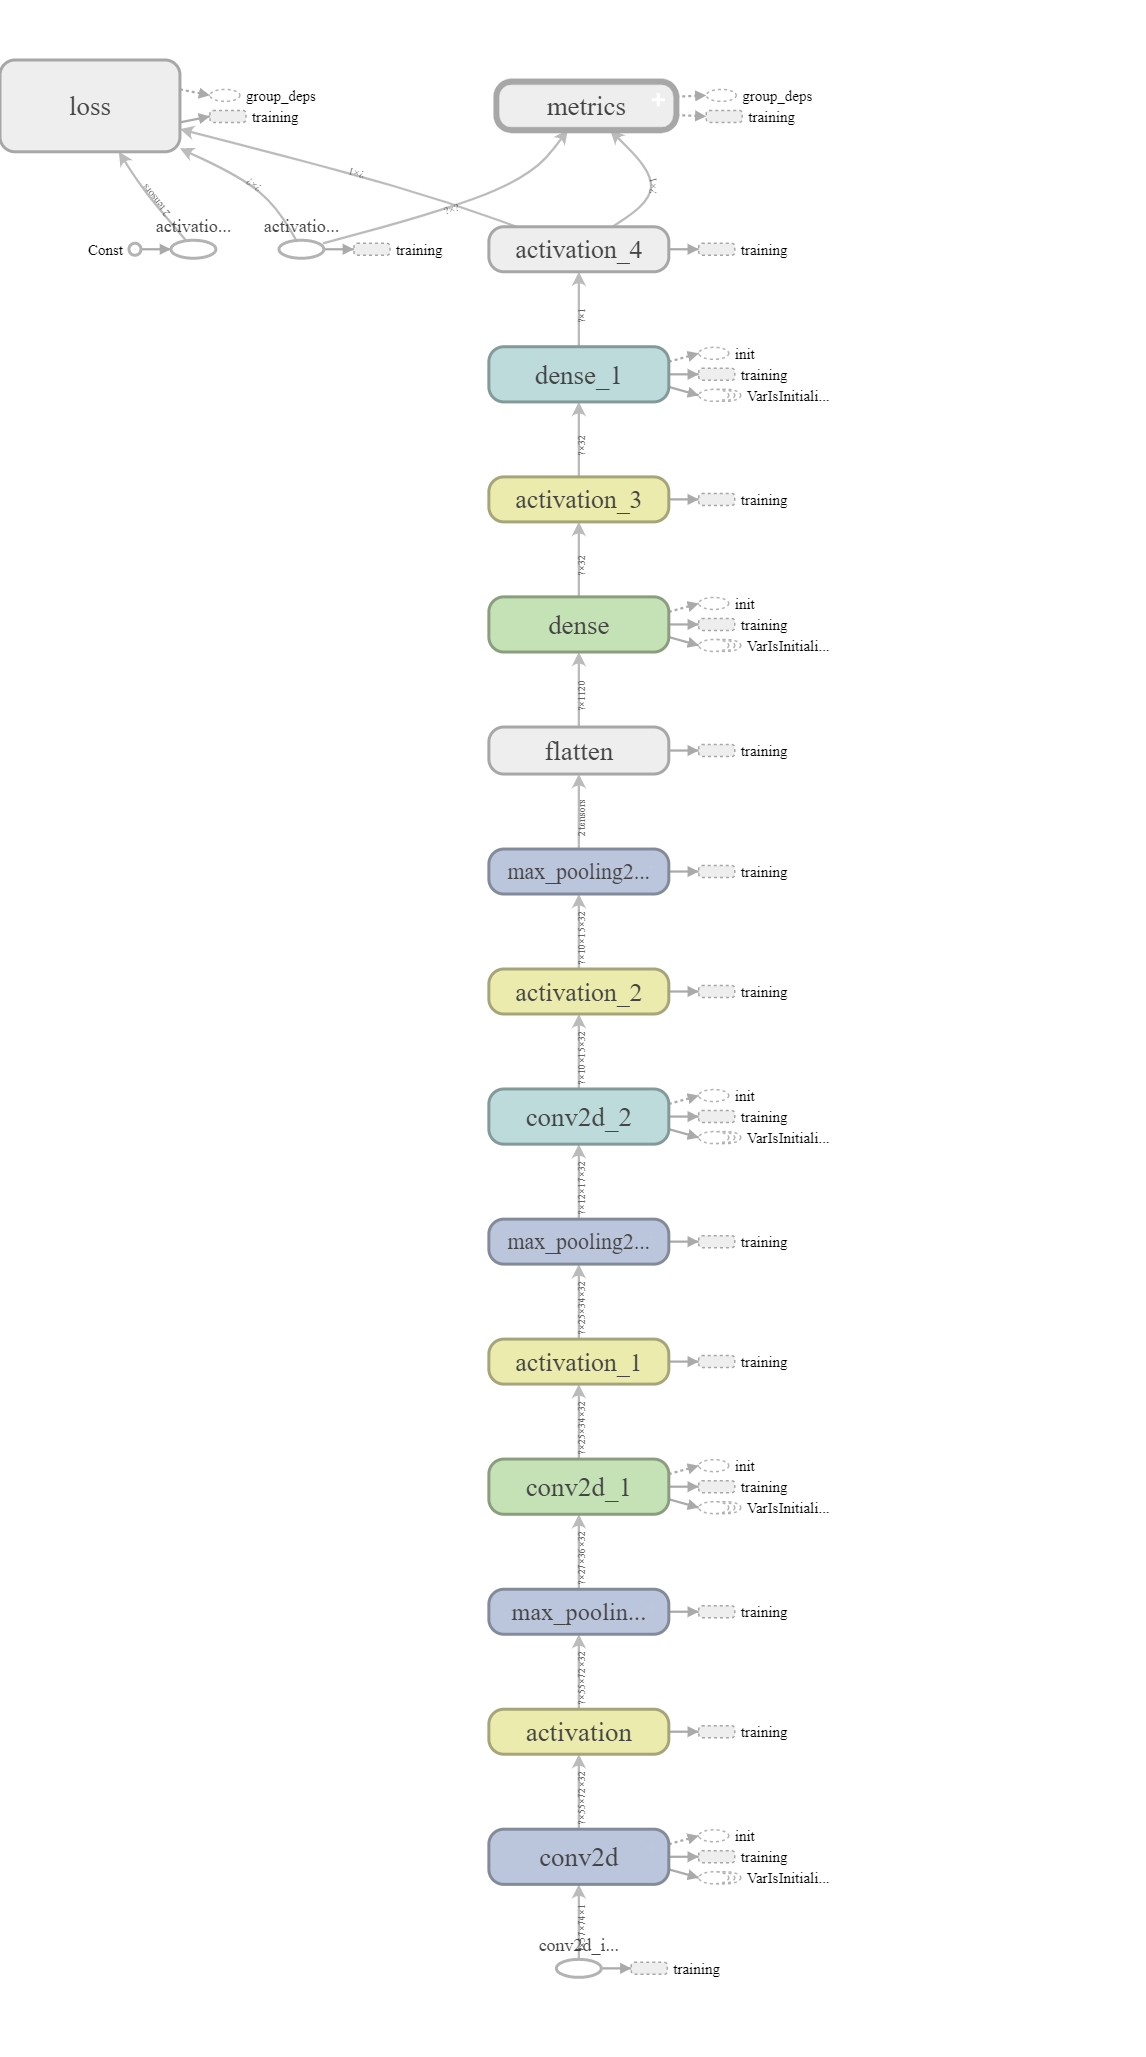
\includegraphics[scale=0.4]{grafo_rete.png}
  \caption{Esempio di grafo di rete prodotto da Tensorboard}
\end{figure}

Le potenzialità di Tensorboard non si limitano soltanto a delle visualizzazioni di grafici tuttavia già solo con questi strumenti si possono andare a comparare i principali parametri e i risultati di vari modelli in modo da capire quale modello si comporta meglio degli altri per il problema in esame.

Nell’elaborato si può abilitare il salvataggio dei log della fase di training, (utilizzati da Tensorboard per costruire i vari grafici) tramite il parametro \texttt{TENSORBOARD} presente nella sezione \texttt{NEURAL\_NETWORK\_TRAIN} del file di configurazione. In questo modo verranno salvati nella sottocartella \texttt{LOGS} di \texttt{MODELS} i logs associati ad ogni modello, poi in Tensorboard sarà possibile selezionare uno o più modelli per visualizzarne tutti i dati.
